\documentclass[10pt]{standalone}
\usepackage{amsmath}
\usepackage{amssymb}
\usepackage{pgf,tikz}
\usepackage{mathrsfs}
\usetikzlibrary{arrows}
\pagestyle{empty}

\begin{document}

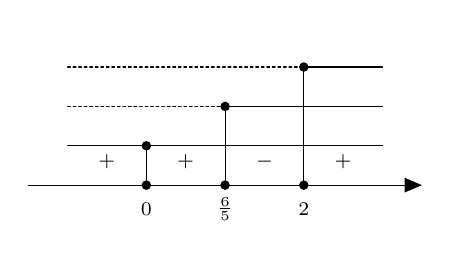
\begin{tikzpicture}[line cap=round,line join=round,>=triangle 45,x=1.0cm,y=1.0cm]

\draw[->,color=black] (-0.5,0.) -- (4.5,0.);

\clip(-0.5,-0.5) rectangle (4.5,2.);
\draw  (0.,0.5)-- (4.,0.5);
\draw  (1.,0.5)-- (1.,0.);
\draw [dash pattern=on 1pt off 1pt]  (0.,1.)-- (2.,1.);
\draw  (2.,1.)-- (4.,1.);
\draw [dash pattern=on 1pt off 1pt] (0.,1.5)-- (3.,1.5);
\draw  (3.,1.5)-- (4.,1.5);
\draw  (2.,1.)-- (2.,0.);
\draw  (3.,1.5)-- (3.,0.);
\begin{scriptsize}
\draw [fill=black] (1.,0.) circle (1.5pt);
\draw(1.0,-0.3) node {$0$};
\draw(0.5,0.3) node {$+$};
\draw(1.5,0.3) node {$+$};
\draw(2.5,0.3) node {$-$};
\draw(3.5,0.3) node {$+$};
\draw [fill=black] (1.,0.5) circle (1.5pt);
\draw [fill=black] (2.,1.) circle (1.5pt);
\draw [fill=black] (2.,0.) circle (1.5pt);
\draw(2.,-0.30) node {$\frac{6}{5}$};
\draw [fill=black] (3.,0.) circle (1.5pt);
\draw(3.0,-0.3) node {$2$};
\draw [fill=black] (3.,1.5) circle (1.5pt);

\end{scriptsize}
\end{tikzpicture}
\end{document}